\documentclass[sigconf,review,screen]{acmart}
% For algorithms in ACM template
\makeatletter
\newif\if@restonecol
\makeatother
\let\algorithm\relax
\let\endalgorithm\relax
\usepackage[ruled,vlined]{algorithm2e}
\usepackage{cleveref}
\usepackage{makecell}
\providecommand\algorithmname{algorithm}

\AtBeginDocument{%
  \providecommand\BibTeX{{%
    \normalfont B\kern-0.5em{\scshape i\kern-0.25em b}\kern-0.8em\TeX}}}

\begin{document}

\title{Compiling Programs to Utilize Cache Optimizations}

\author{Samuel Grayson}
\email{grayson5@illinois.edu}
\affiliation{%
  \institution{University of Illinois at Urbana-Champaign}
}

\author{Nirupam K N}
\email{nirupam2@illinois.edu}
\affiliation{%
  \institution{University of Illinois at Urbana-Champaign}
}

\settopmatter{printacmref=false} % Removes citation information below abstract
\renewcommand\footnotetextcopyrightpermission[1]{} % removes footnote with conference information in first column

\newcommand{\todo}[1]{\textcolor{red}{#1}}

\begin{abstract}
In most state-of-the-art systems, the cache coherence pattern has been fixed in architecture, which does not know about the general structure of the program it is executing.
However, Spandex changes supports the possibility of dynamically selected cache coherence optimizations.
We exploit this opportunity by writing a compiler-pass that analyzes the memory-access pattern in parallel tasks and selects a specialized cache coherence pattern.
\end{abstract}

% http://dl.acm.org/ccs.cfm
\begin{CCSXML}
<ccs2012>
<concept>
<concept_id>10010520.10010521</concept_id>
<concept_desc>Computer systems organization~Architectures</concept_desc>
<concept_significance>500</concept_significance>
</concept>
<concept>
<concept_id>10011007.10011006.10011041</concept_id>
<concept_desc>Software and its engineering~Compilers</concept_desc>
<concept_significance>500</concept_significance>
</concept>
</ccs2012>
\end{CCSXML}
\ccsdesc[500]{computer systems organization~Architectures}
\ccsdesc[500]{Software and its engineering~Compilers}

\keywords{cache coherence, heterogeneous systems, compilers}

\maketitle

\section{Introduction}

Many multi-processor systems use the MESI protocol for cache coherence \cite{Primer_on_Memory_Consistency}, which provides sequential consistency for any data race-free program. However, the cache coherence protocol might make redundant or indirect requests because it does not know about the program structure.

For example, suppose a program directs each processor to compute one layer of a neural net in a pipelined fashion (see \cref{fig:pipelined_net}). Processor \(i\) needs to send its activation's to Processor \(i+1\) so that Processor \(i+1\) can compute the next layer of activations. In traditional MESI system, Processor \(i\) would store data to its cache, in `exclusive' state. Then Processor \(i+1\) would attempt to load the data, miss in its cache, go to the bus, ask Processor \(i\) for data, downgrading \(i\)'s copy to `shared' state.

\begin{figure}[h]
  \centering
  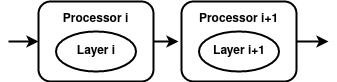
\includegraphics[width=0.375\textwidth]{pipelined_parallelism.png}
  \caption{The dataflow graph of pipelined neural net inference}
  \Description{Dataflow graph where Processor \(i\) computes layer \(i\) and sends activations to Processor \(i+1\).}
  \label{fig:pipelined_net}
\end{figure}

An optimization is available: The compiler could prove that Processor \(i+1\) is the consumer of the activations written by Processor \(i\), so it could instruct Processor \(i\) to send its data directly to the cache of Processor \(i+1\), bypassing the Last-Level Cache (LLC) \cite{DeNovo}.  Streaming programs spend a substantial portion of their time and energy in the Network on Chip (NoC), so optimizations like this save power and time \cite{dynamic_cache_coherence}.

Many of these coherence optimizations are only beneficial in specific cases, so the architecture needs to dynamically select the best coherence optimization for the given memory-locations based on the access pattern while maintaining correctness. The architecture only knows about historical access patterns and does not know what the other processors in the system are doing, so it is difficult for the architecture to select a coherence optimization by itself. The compiler can form an expectation of future access patterns and could know what other processors in the system are doing, so it should inform the architecture what coherence optimization to use for specific memory-locations.

Our contribution is a compiler-pass which analyzes the access pattern of the given program to identify certain opportunities for coherence optimization. We hope future work will build on this pass to support more kinds of coherence optimizations and develop a better cost-model. Our implementation leverages the HPVM compiler Intermediate Representation (IR) \cite{HPVM} and emits coherence optimizations for the Spandex Cache Coherence protocol \cite{Spandex}.
\section{Related Work}
\label{related_work}

Remote Store Programming \cite{remote_store_programming} exploits a similar data-movement optimization, but it requires manual programmer input. The goal of this work is to automate that analysis. While future versions of this compiler could target RSP, targeting Spandex gives us a superset of the optimizations available in RSP.

Prior work on DeNovo cache coherence protocol does include a compiler. Still, it assumes programs are written in a language with annotated memory-effect regions (for each function, a set of memory locations which it could read and another set which it could write) \cite{DeNovo}. No popular programming language includes manual annotations; manual annotations are too tedious and error-prone to burden computer programmers. Despite the plethora of work \cite{effect_and_effect_inference_java,polymorphic_effect_systems,OO_effect_system} on memory-effect inference, no popular language tool-chain includes such an inference pass; they are expensive to perform on an imperative language with polymorphism. 
Work on dynamic cache-coherence in Spandex \cite{dynamic_cache_coherence} presents a high-level algorithm, but it is too high-level for a compiler-developer to implement directly. 
\section{Implementation}

\subsection{Coherence Optimizations}

Most coherence protocol do not support dynamically selecting coherence optimizations (as discussed in \cref{related_work}).
Spandex \cite{Spandex} is one which does, and dynamic coherence optimizations have already been suggested in prior work \cite{dynamic_cache_coherence}.

In Spandex, there are four states: \textit{Invalid}, \textit{Valid} (read-only copy expecting self-invalidation), \textit{Shared} (read-only copy expecting writer-invalidation), and \textit{Owned} (writable with no invalidation messages).

To limit the scope of coherence optimizations, we will consider the special case of producer/consumer relationships, where the producer issues and completes all stores before the consumer issues and completes all loads every epoch, and this pattern repeats. This is a widespread paradigm in pipelined parallelism, such as recurrent neural net training and inference.

\textbf{MESI:} In MESI, initially all lines would be invalid-state. The producer's first store to a line issues an invalidation on the bus and moves the line into modified-state. Subsequent stores hit. The consumer's first load to a line requests this line from the producer, moving both copies into shared-state.

\textbf{Spandex:} Without optimization, the Spandex coherence protocol emulates this, except the L2 is directory-based not bus-based, so the invalidation request looks up any processors which hold the line.

\textbf{Spandex Producer-Owned:} One possible optimization is to have the producer always own the buffer, so all of its stores hit locally. The consumer would have to look the line up in the producer's cache, but the owner can be predicted in hardware (suggested in \cite{dynamic_cache_coherence}), so this request goes from L1-to-L1 (bypassing the L2).
%\footnote{One may be concerned about memory consistency, if data can change while the consumer is loading it. Such a program would already have synchronization forcing the producer to `happen-before' the consumer to be correct in the first place. This existing synchronization is sufficient to maintain memory consistency. Waiting on this synchronization not limit the degree of parallelism, because th producer can be working on a second input datum in a double-buffered fashion.}
The compiler would insert a self-invalidation request in the consumer's code at the end of every epoch, to maintain memory consistency.
This is optimal when the loads are sparse, because traffic is only generated for each load.

\textbf{Spandex Consumer-Owned:} Another possible optimization is to have the consumer always own the buffer, so all of its loads hit locally, as suggested in \cite{dynamic_cache_coherence}. The producer would writethrough with owner prediction, allowing it to send data directly to the consumer's cache.
This is optimal when the write are sparse, because traffic is only generated for each write and there is little memory parallelism. No computation of the producer is logically dependent on store, but much of the consumer's computation may be logically dependent on the result of a load, so increasing the latency of stores in exchange for decreasing the latency of loads can be desirable.

\subsection{Identifying Producer/Consumer Relationships}

In order to identify the memory access pattern among multiple parallel tasks, we need an Intermediate Representation (IR) that takes task-level parallelism into account. Traditional compiler IRs like LLVM \cite{LLVM} and GIMPLE \cite{GIMPLE} do not support this, for example. HPVM is an extension of LLVM that represents task- and data-parallelism \cite{HPVM}. Currently, HPVM programs are written in C with library calls, which is a cumbersome interace, but there are plans to add a frontend to higher-level languages such as Keras.

In HPVM, programs are represented as a hierarchical dataflow graph (DFG). Every node is either called a `leaf' or an `internal' node. For example in \cref{fig:hierarchical_dfg} C, E, and F are leaves, while A, B and D are internal.

Leaf nodes can contain computation while internal nodes can only string together other nodes. HPVM can execute one input at a time, in which case the parallelism is the width of the DFG, but HPVM  also supports `streaming' (pipelined) execution, where time can be divided into epochs where every node runs once each epoch and the parallelism is the number of nodes in the DFG. In each epoch, every node runs on its own data-item, passing data to its successors to compute on in the next epoch. The data passed through pointers between nodes every epoch is exactly the kind of repeated producer/consumer relationship that we want to optimize.

We want to detect any loads and stores in different nodes that refer to the same memory location. Therefore, we trace each pointer from its definition to its use.
Initially, our pass will assign all producer/consumer memory accesses to a given coherence optimization.
In the future, our compiler-pass would examine the memory access-pattern on these pointers.

\subsection{Access-Pattern Analysis}

HPVM gives us a hierarchical DFG graph (see \cref{fig:hierarchical_dfg}). The first step is to flatten the graph, so we see how data is passed between the leaves (see \cref{fig:flattened_dfg}). This is done by \cref{algo:flatten_dfg}. 

\begin{figure}[h]
    \centering
    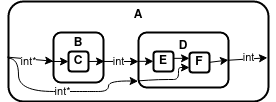
\includegraphics[width=0.45\textwidth]{hierarchical_dfg.png}
    \caption{Hierarchical DFG}
    \Description{Letters are nodes. At the first level, A contains B and D. At the second level, B contains C (leaf), while D contains E (leaf) and F (leaf).}
    \label{fig:hierarchical_dfg}
\end{figure}

\begin{algorithm}[h]
%\SetAlgoLined
\SetKwInOut{Input}{input}
\SetKwInOut{Output}{output}

\SetKwData{hdfg}{hdfg}
\SetKwData{fdfg}{fdfg}
\SetKwData{source}{source}
\SetKwData{destination}{destination}

\Input{a hierarchical DFG, \hdfg}
\Output{a flat DFG, \fdfg}
 \For{\source in \hdfg nodes}{
  \eIf{\source is leaf}{
    \(\source' := \source\)
  }{
    \(\source' := \source.\mathrm{entry}\), where \source.{entry} is a dummy node bearing that name. It will be removed later.\;
  }
  \For{\destination, where \(\source \to \destination\) in \hdfg}{
    \eIf{\destination is leaf}{
      \(\destination' := \destination\)\;
    }{
      \(\destination' := \destination.\mathrm{entry}\)\;
    }
    Insert \(\source' \to \destination'\) into \fdfg\;
  }
 }
 \caption{Flattening the HPVM DFG}
 \label{algo:flatten_dfg}
\end{algorithm}

\begin{figure}[h]
    \centering
    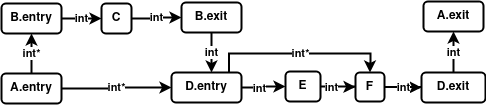
\includegraphics[width=0.49\textwidth]{flattened_dfg.png}
    \caption{Flattened DFG}
    \Description{A.entry to B.entry to C to B.exit to D.entry to F to E to D.exit to A.exit. In parallel, A.entry to D.entry. In parallel, D.entry to E}
    \label{fig:flattened_dfg}
\end{figure}

Next, we need to expose the leaf-connectivity (see \cref{fig:leaf_dfg}), because the leaves are the nodes which contain all computation, including loads and stores. This is done by \cref{algo:leafen_dfg}.

\begin{algorithm}[h]
%\SetAlgoLined
\SetKwInOut{Input}{input}
\SetKwInOut{Output}{output}

\SetKwData{ldfg}{ldfg}
\SetKwData{fdfg}{fdfg}
\SetKwData{node}{node}
\SetKwData{predecessor}{predecessor}
\SetKwData{successor}{successor}

\Input{a flat DFG, \fdfg}
\Output{a leaf DFG, \ldfg}
Initialize \ldfg to a copy of \fdfg\;
\For{\node \(\in\) \fdfg}{
  \If{\node is not a leaf and not the root entry/exit}{
    \For{\(\predecessor \to \node, \node \to \successor \in \ldfg\)}{
      Remove \(\predecessor \to \node\) from \ldfg\;
      Remove \(\node \to \successor\) from \ldfg\;
      Insert \(\predecessor \to \successor\) into \ldfg\;
    }
  }
}
\caption{Pruning non-leaves from the flat DFG}
\label{algo:leafen_dfg}
\end{algorithm}

\begin{figure}[h]
    \centering
    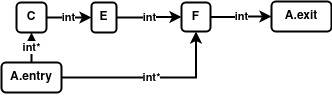
\includegraphics[width=0.4\textwidth]{leaf_dfg.png}
    \caption{Leaf Dataflow Graph}
    \label{fig:leaf_dfg}
\end{figure}

Finally, we need to look through the leaf DFG and determine where there is implicit memory communication (see the memory communication graph in \cref{fig:mem_comm_dfg}). This is done by \cref{algo:mem_comm_dfg}.

\begin{algorithm}[h]
%\SetAlgoLined
\SetKwInOut{Input}{input}
\SetKwInOut{Output}{output}

\SetKwData{ldfg}{ldfg}
\SetKwData{mcdfg}{mcdfg}
\SetKwData{node}{node}
\SetKwData{A}{A}
\SetKwData{B}{B}
\SetKwData{predecessor}{predecessor}
\SetKwData{successor}{successor}

\Input{a leaf DFG, \ldfg}
\Output{a memory-communication DFG, \mcdfg}

Initialize \ldfg to a copy of \mcdfg\;
\For{\(\node \in \ldfg\)}{
  \If{\node emits a pointer type}{
    \For{\(\node \to \A, \node \to \B \in \ldfg\)}{
      \If{Pointer is writable in \A and \A precedes \B}{
        Insert \(\A \to \B\) into \mcdfg\;
      }
    }
  }
}
\caption{Pruning non-leaves from the flat DFG}
\label{algo:mem_comm_dfg}
\end{algorithm}

\begin{figure}[h]
    \centering
    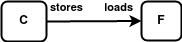
\includegraphics[width=0.3\textwidth]{mem_comm_dfg.png}
    \caption{Memory Communication Graph}
    \label{fig:mem_comm_dfg}
\end{figure}

Finally, we have analyzed the memory access-patterns in the program and identified consumer/producer relationships for cache optimization. Future work would do even more analysis on these relationships.
\section{Methods}
\label{sec:methods}

Unfortunately, there is only one existing simulator or Spandex protocol, and it is not possible to set up in such a short period of time. There are students working on a gem5 simulator, but that effort was not ready when we were like we had hoped. As such, the experiments in this report will depend on analytical models.

We have annotated each benchmark so that it logs all loads and stores to the buffers I am considering a part of the producer/consumer relationship. Then, we wrote a program that simulates the cache states for those addresses. These are the assumptions our simulator makes:

\begin{itemize}
    \item If the coherence optimization supports coalescing and a store is to the same line as one of the previous \(N\) stores (where \(N\) is a parameter defined below), it gets coalesced.
    \item The program is in steady-state (no cold-effects). We \textit{do} simulate cold-effects which would recur at the beginning of every epoch. 
    \item The working-set fits in the L1 cache. No conflict or capacity misses.
\end{itemize}

The parameters we used are detailed in \cref{table:params}. The latency numbers come from a prior publication on dynamic cache coherence \cite{dynamic_cache_coherence} and the flit sizes come from the RTL implementation of Spandex, which in turn is dictated by ESP \cite{ESP}.

\begin{table}[h]
  \caption{Simulation parameters}
  \label{table:params}
  \begin{tabular}{cc}
  \toprule
  \textbf{Parameter} & \textbf{Value} \\
  \midrule
  Avg. hops from L1 to peer L1 & 1.0 hops \\
  Avg. hops from L1 to L2 & 1.0 hops \\
  Avg. hops from L1 to bus & 1.0 hops \\
  Write coalescing buffer size & 32 entries \\
  L1 hit & 1 cycle \\
  Avg. latency of L1 to peer L1 and back & 60 cycles \\
  Avg. latency of L1 to L2 to peer L1 and back & 80 cycles \\
  Avg. latency of  L1 to bus to peer L1 and back & 70 cycles \\
  Word size & 1 flit \\
  Address size & 1 flit \\
  Header size & 1 flit \\
  Line size & 8 words \\
  \bottomrule
\end{tabular}
\end{table}

We annotated these three benchmarks:

\begin{itemize}
    \item \verb+rw+ a microbenchmark with 2 stages, where the producer writes to every byte in a buffer, and the consumer reads all of the writes.
    \item \verb+sparse_rw+ like \verb+rw+, but producer and consumer only access the first word of every line. This is representative of a ``sparse'' data access pattern, which eliminates the effect of coalescing.
    \item \verb+ed+ an edge-detection pipeline with 5 stages pipeline with 2 parallel paths. This example exhibits pipeline-parallelism and task-parallelism.
    \item \verb+cava+ Harvard Camera image processing pipeline, with 7 stages. This is a good example of a realistic application.
\end{itemize}

We considered annotating parboil benchmarks, but they do not naturally exhibit pipelined parallelism, as they are more a test of data-parallelism, so it does not fit the producer/consumer model as well.

The cost model we use is described in \cref{table:costs}. Note the last case (Spandex consumer-owned loads) are where write coalescing becomes relevant. All words written to a line can piggy-back off of the same packet.

\begin{table*}[h]
  \caption{Latency and network cost of each request in terms of the parameters above.}
  \label{table:costs}
  \begin{tabular}{cccccc}
  \toprule
  \textbf{Scenario} & \textbf{Request} & \textbf{State} & \textbf{State Change} & \textbf{Latency} & \textbf{Traffic Routed} \\
  \midrule
  MESI & store & S & \makecell[tc]{issuer to M \\ others to I} & L1-bus-peerL1-L1 &
    \makecell[tc]{2 \(\times\) (L1 to L2 hops) \(\times\) (Inv: header + address) \\ + (L1 to L1 hops) \(\times\) (InvAck: header + address)} \\
   & store & M & M & L1 hit & 0 \\
   & load & I & all to S & L1-bus-peerL1-L1 &
    \makecell[tc]{2 \(\times\) (L1 to Bus hops) \(\times\) (ReqS: header + address) \\ + (L1 to L1 hops) \(\times\) (RspSdata: header + address + line)} \\
   & load & S & S & L1 hit & 0 \\
\midrule
  Spandex & store & S & \makecell[tc]{issuer to O \\ others to I} & L1-L2-peerL1-L1 &
    \makecell[tc]{2 \(\times\) (L1 to L2 hops) \(\times\) (Inv: header + address) \\ + (L1 to L1 hops) \(\times\) (InvAck: header + address)} \\
   & store & O & O & L1 hit & 0 \\
   & load & I & all to S & L1-L2-peerL1-L1 &
    \makecell[tc]{2 \(\times\) (L1 to L2 hops) \(\times\) (ReqS: header + address) \\ + (L1 to L1 hops) \(\times\) (RspSdata: header + address + line)} \\
   & load & S & S & L1 hit & 0 \\
\midrule
  \makecell[tc]{Spandex \\ prod.-owned} & store & O & O & L1 hit & 0 \\
   & load & I & V & L1-peerL1-L1 &
  \makecell[tc]{(L1 to L1 hops) \(\times\) (ReqV: header + address) \\ + (L1 to L1 hops) \(\times\) (RspData: header + address + line)} \\
   & load & V & V & L1 hit & 0 \\
\midrule
  \makecell[tc]{Spandex \\ cons.-owned} & store & I & I & L1-peerL1-L1 &
  \makecell[tc]{(L1 to L1 hops) \(\times\) (ReqWTo: header + address + data) \\ + (L1 to L1 hops) \(\times\) (AckWT: header + address)} \\
   & load & O & O & L1 hit & 0 \\
  \bottomrule
\end{tabular}
\end{table*}
\section{Experimental Results}

\begin{figure}[h]
    \centering
    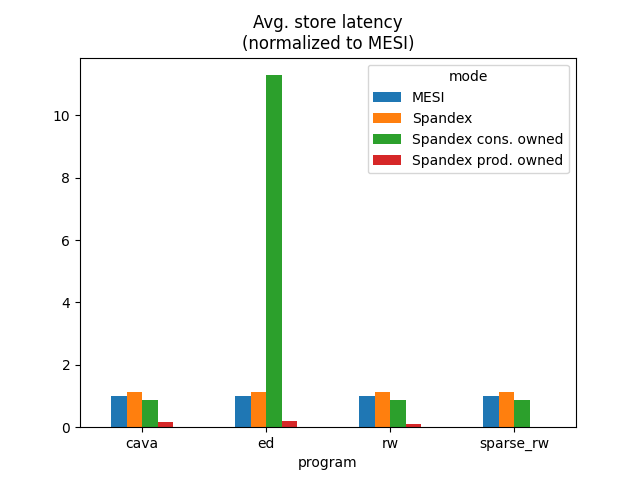
\includegraphics[width=0.45\textwidth]{stores.png}
    \caption{Average Store Latency}
    \label{fig:stores}
\end{figure}

\begin{figure}[h]
    \centering
    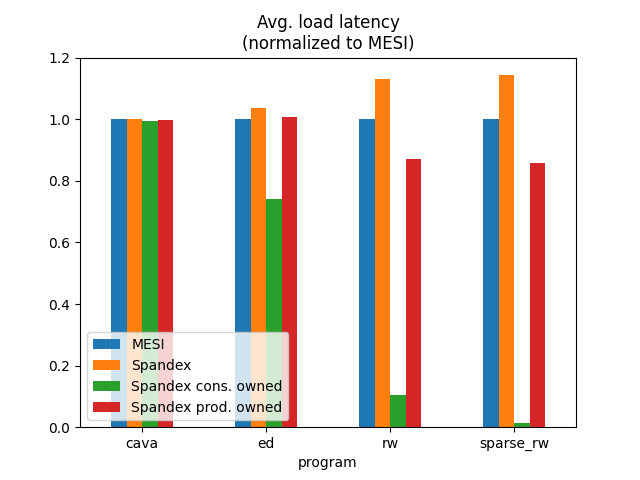
\includegraphics[width=0.45\textwidth]{loads.png}
    \caption{Average Load Latency}
    \label{fig:loads}
\end{figure}

\begin{figure}[h]
    \centering
    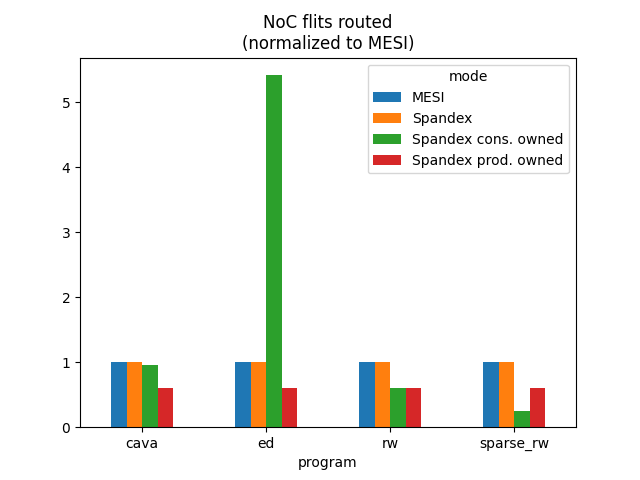
\includegraphics[width=0.45\textwidth]{traffic.png}
    \caption{NoC Traffic Routed}
    \label{fig:traffic}
\end{figure}

Average store latency is least with Spandex producer-owned lines while load latency is least with Spandex consumer-owned lines, both as expected. However, the magnitude of the effect varies widely with the application, by what we believe to be the sparsity of loads relative to the sparsity of stores. NoC usage is least for better for Spandex consumer-owned when the accesses are sparse, and Spandex producer-owned when they are dense.

We believe \verb+ed+ suffers high NoC traffic with Spandex consumer-owned (\(\sim\)10x MESI case) because it has several for-loops that cut `against the grain', so the stores are unable to be coalesced. However, MESI can still exploit reuse, because it brings the whole line to the writer, so future writes to that line hit \textit{for the duration of the epoch, instead of for the duration of the coalescing window}.

Currently, our compiler pass would select the same kind of request-type mapping for all producer/consumer relationships, so we would select a good all-around cache optimization, like producer-owned for these accesses. This is still dynamic in the sense that accesses outside of the producer/consumer relationship will be regular Spandex requests, while producer/consumer accesses are optimized. However, future work could look at the sparsity of loads and stores and decide for each producer/consumer pair which cache optimization to apply. The benchmarks we ran indicate that when trying to optimize NoC traffic, some cases  (\verb+cava+, \verb+ed+, and \verb+rw+) would want producer-owned, but others (\verb+sparse_rw+) would want consumer-owned. NoC traffic routed correlates well with energy utilization, as much of the energy is spent in the interconnect, so this optimization is important for low-power devices \cite{low_energy_FPGA}. Optimizing for runtime, however, is somewhat more nuanced due to parallelism.

We do not know exactly how the load-latency and store-latency effects the runtime of each benchmark, and we could not simulate the benchmarks for the reasons outlined in \cref{sec:methods}. The effect of store-latency is partially isolated by the MSHR buffer. It is probable that \verb+ed+ has such a large average store latency that it would fill the MSHR and induce stalls. The impact of load-latency on runtime is also not straightforward because the processor may be able to execute independent instructions out-of-order while waiting for a load. However, many important programs are memory-bound, so these would be sensitive to the load-latency. For example, linked-list traversals would be strongly affected by load-latency.
\section{Future Work}
Future work could try to estimate the sparsity of stores compared to the sparsity of loads. Since we have identified the leaf nodes containing the producing and consuming logic, one can use the LLVM analysis tools \cite{LLVM} to ask how many times a static instruction will be run (trip count). Even if this only applied in cases where the code path is statically knowable, a lot of SGEM and image processing code has this property. Then, one could either assume memory accesses are uniform across the buffer or do even more detailed analysis to determine how many accesses are to unique lines in the buffer. Our experiments show there could be extreme benefits in being able to select cache optimization for each access pattern.

We focused entirely on the data-movement between leaves, but future work might optimize the synchronization logic in the HPVM runtime as well. Furthermore, one might also want to look at more kinds of cache optimizations.

Finally, when a simulator becomes available, future work should utilize a proper architectural simulation to produce actual runtime improvement estimates.
\section{Conclusion}

Our experiments show modest gain in certain architectural metrics through compiler-guided cache optimization. More serious gains are within reach, by selecting a different request type mapping for each producer/consumer instead of the same for all.

\begin{acks}
We would like to acknowledge John Alsop and Sarita Adve. It was invaluable to have feedback and input from the authors of the work we build on \cite{Spandex,dynamic_cache_coherence}.
\end{acks}

%%
%% The next two lines define the bibliography style to be used, and
%% the bibliography file.
\bibliographystyle{ACM-Reference-Format}
\bibliography{main}

% \appendix
% \section{Research Methods}
% \subsection{Part One}

\end{document}
\endinput